\chapter{Anexo B: Manual de Usuario}

La mayoria de las tareas que realiza este sistema de video-vigilancia inteligente son automáticas, pero las tareas más basicas a describir son las siguientes:

% \begin{enumerate}
%     \item Conectar cámara
%     \item Desconectar cámara
%     \item Recibir notificaciones
% \end{enumerate}
\section*{Conectar cámara}
Para conectar una nueva cámara es necesario tener el servidor-TCP funcionando. Para levantas una nueva instancia de cámara se siguen los siguientes pasos:
\begin{enumerate}
    \item En el directorio donde se desplego el módulo de cámaras ejecutar el siguiente comando:\begin{center}
        \shellcmd{./run.sh}
    \end{center}
    \item De acuerdo a la configuración del servidor-TCP ingrerar los valores de dirección y puerto en el formato siguiente:
    \begin{itemize}
        \item Dirección : 0.0.0.0 hasta 255.2555.255.2555
        \item Puerto: Desde 49152 hasta 65535
        \item ID Cam: valor numérico para el identificador
    \end{itemize}
    Definir estos valores en los campos correspondientes:
    \begin{figure}[H]
        \begin{center}
            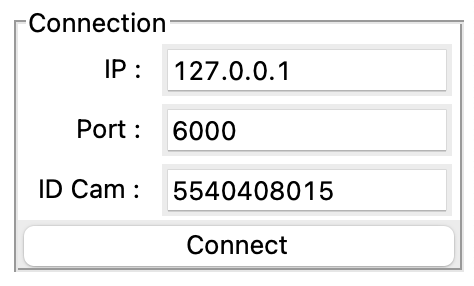
\includegraphics[width=5cm]{img/anexos/ip_port.png}
            % \caption{Interfaz del módulo de cámaras.}
            % Fuente : Elaboración propia
        \end{center}
    \end{figure}
    
    \item En el panel de controles se tiene 3 opciones para iniciar el módulo antes de conectarse:
        \begin{itemize}
            \item[A]: Iniciar cámara web integrada o externa.
            \item[B]: Iniciar PiCámara, solo si esta disponible en un equipo RaspberryPi.
            \item[C]: Iniciar Video, en caso de solo contar con grabaciones.  
        \end{itemize}
    \begin{figure}[H]
        \begin{center}
            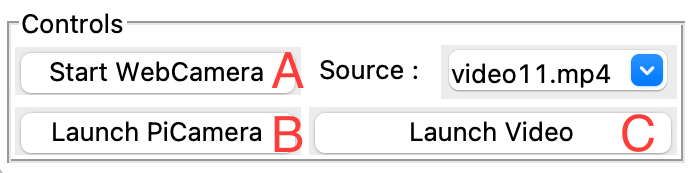
\includegraphics[width=10cm]{img/anexos/controls_camera.png}
            % \caption{Interfaz del módulo de cámaras.}
            % Fuente : Elaboración propia
        \end{center}
    \end{figure}
    Se elige una de esas opciones según al requerimientos del usuario.
    \item Presionar el boton ``Conectar'' y se empezará a enviar los fotogramas de video.
    \begin{center}
        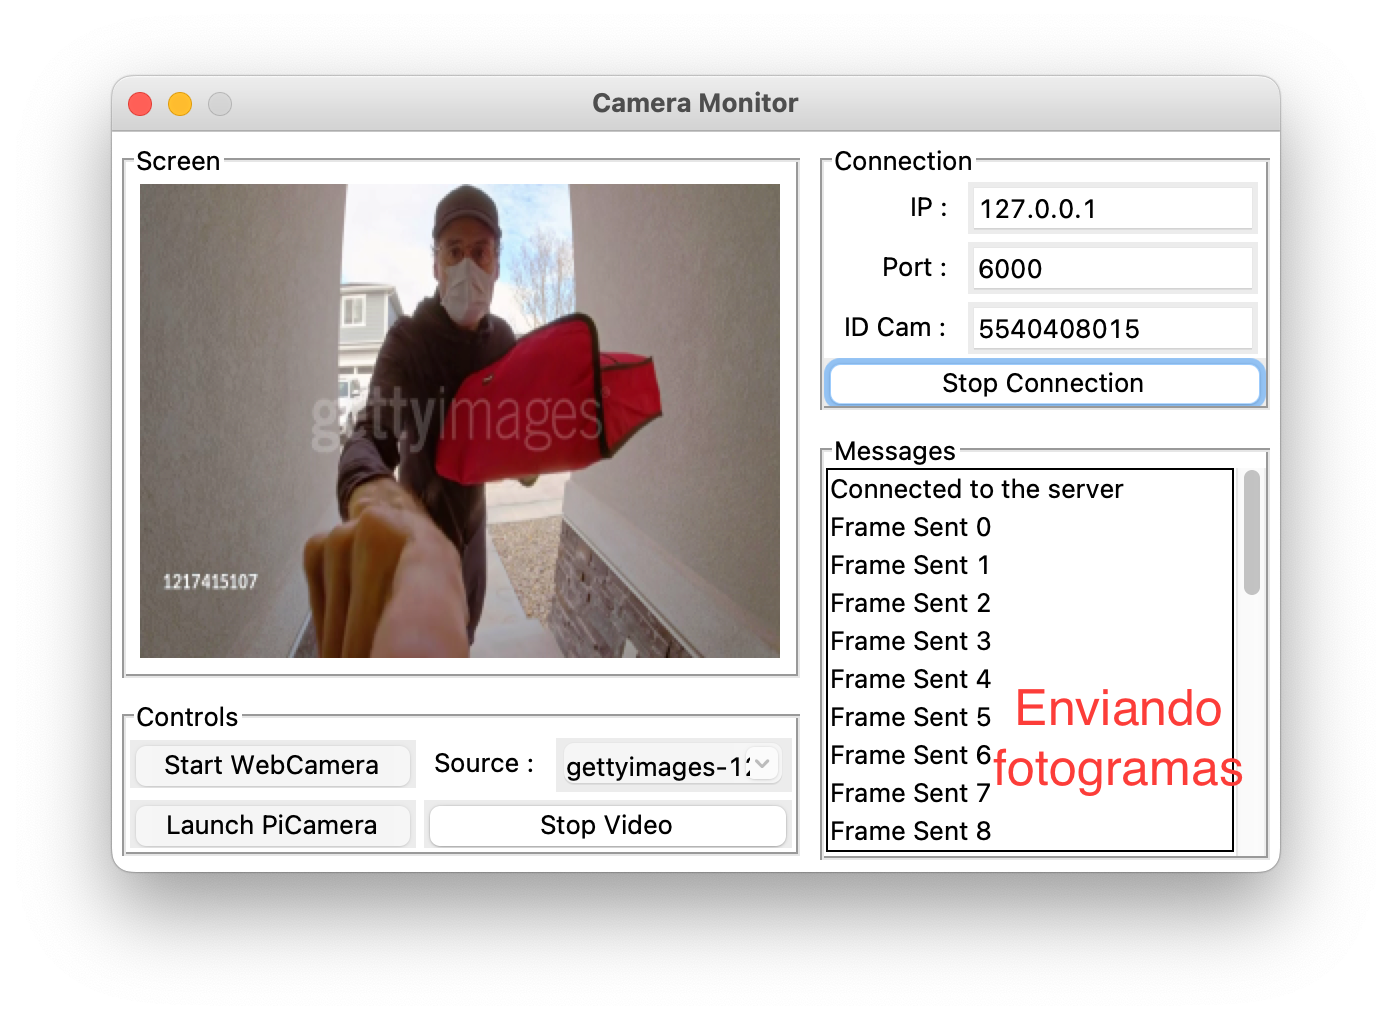
\includegraphics[width=10cm]{img/anexos/send_frames.png}
        % \caption{Interfaz del módulo de cámaras.}
        % Fuente : Elaboración propia
    \end{center}
    
\end{enumerate}

\section*{Desconectar cámara}

Cuando se tiene una cámara ejecutando el envion de fotogramas, es posible que el usuario quiera desconectarl. Para este objetivo se siguen los siguientes pasos.
\begin{enumerate}
    \item Parar la conección presionando en el botón: ``Stop Connection''.
    \begin{center}
        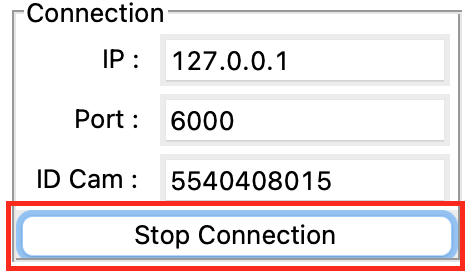
\includegraphics[width=5cm]{img/anexos/stop_connection.png}
        % \caption{Interfaz del módulo de cámaras.}
        % Fuente : Elaboración propia
    \end{center}
    \item En caso de querer apagar la cámara se debera presionar en su debido botón la opcion de ``Parar Cámara''
    \begin{center}
        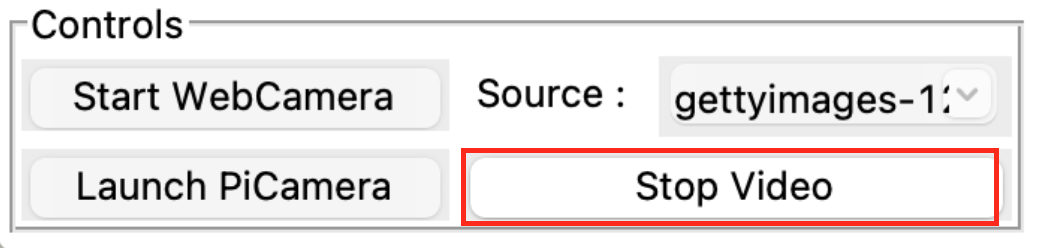
\includegraphics[width=10cm]{img/anexos/stop_video.png}
        % \caption{Interfaz del módulo de cámaras.}
        % Fuente : Elaboración propia
    \end{center}
\end{enumerate}

\section*{Visualizar transmisión de video en vivo}
Para la visualización del video en vivo se recibe un correo eléctrónico con el enlace directo a la transmisión.

Para reproducir esta transmisión se debe seguir los siguientes pasos:
\begin{enumerate}
    \item Revisar el correo electrónico correspodiente a la conexión.
    \begin{center}
        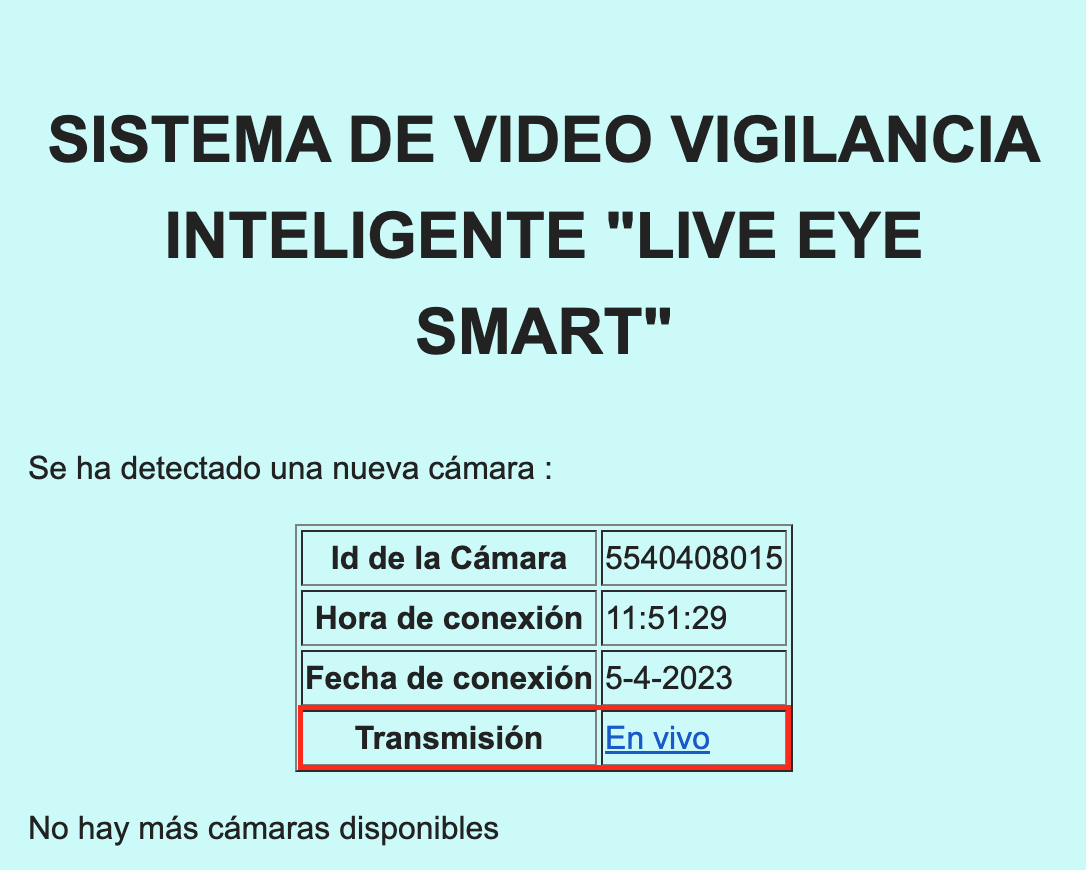
\includegraphics[width=10cm]{img/anexos/link.png}
        % \caption{Interfaz del módulo de cámaras.}
        % Fuente : Elaboración propia
    \end{center}
    \item Redirigirse al enlace de transmisión.
    \begin{center}
        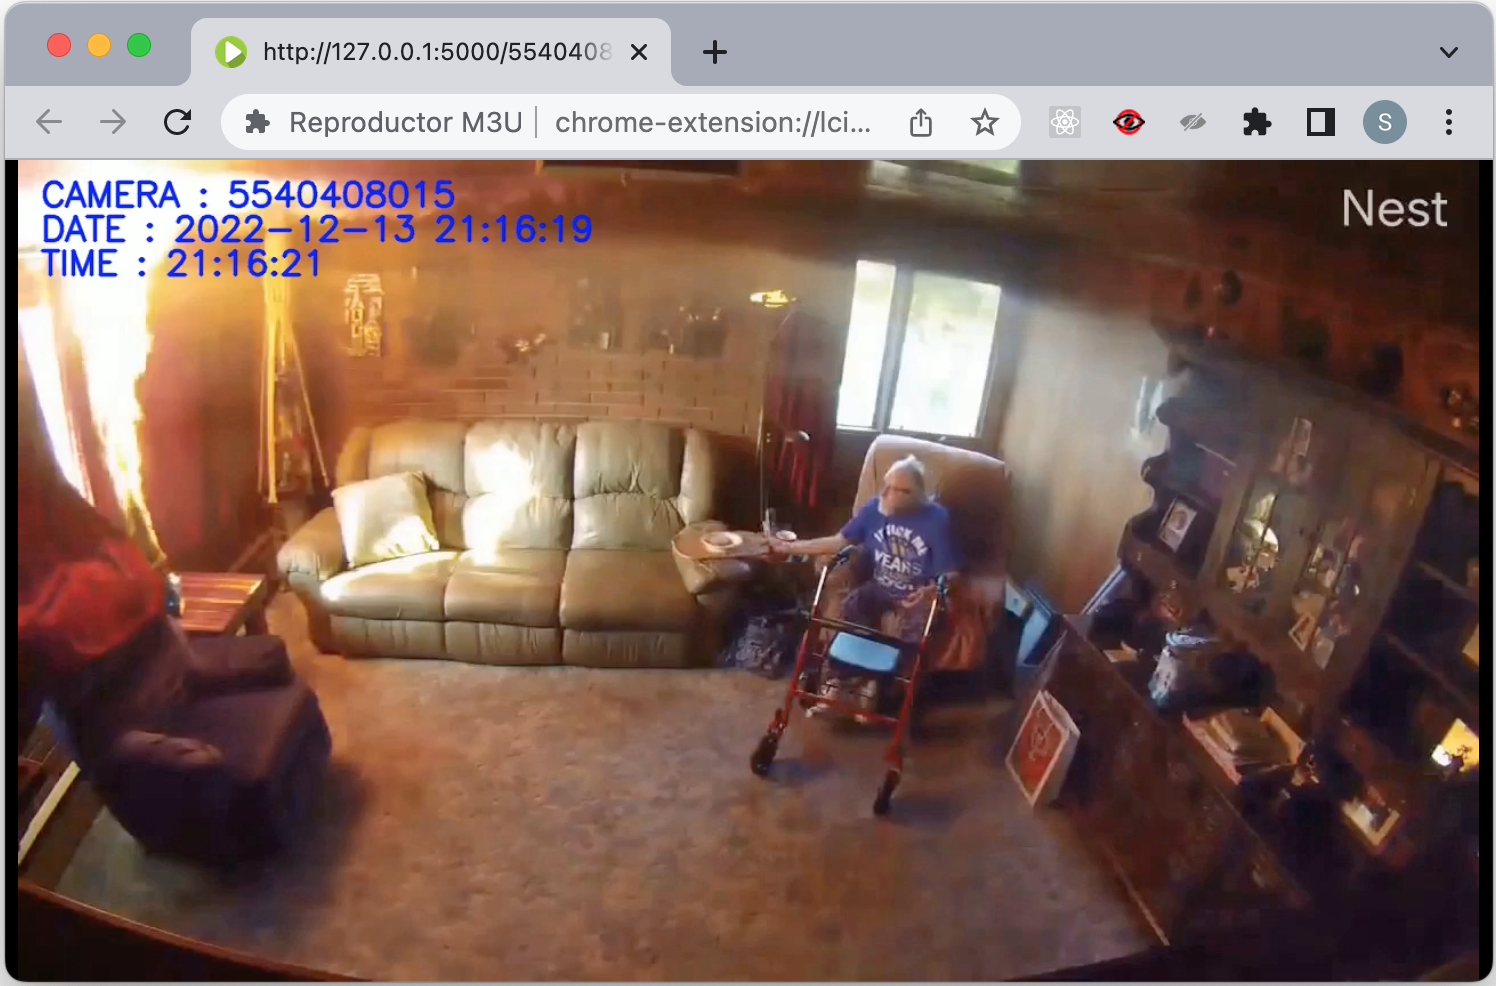
\includegraphics[width=10cm]{img/anexos/stream_web.png}
        % \caption{Interfaz del módulo de cámaras.}
        % Fuente : Elaboración propia
    \end{center}
\end{enumerate}